\documentclass[a4paper,12pt]{article}

% ----------------- Encoding -----------------
\usepackage[utf8]{inputenc}
\usepackage[T1]{fontenc}
\usepackage{lmodern}

% ----------------- Math -----------------
\usepackage{amsmath, amssymb, amsfonts, bm}

% ----------------- Figures -----------------
\usepackage{graphicx}
\usepackage{float}

% ----------------- Tables -----------------
\usepackage{booktabs}

% ----------------- Graphics (TikZ) -----------------
\usepackage{tikz}
\usetikzlibrary{arrows.meta, positioning, shapes.geometric}

% ----------------- Page layout -----------------
\usepackage{geometry}
\usepackage{hyperref}
\geometry{margin=2.5cm}
\setlength{\parskip}{6pt}
\setlength{\parindent}{0pt}

\title{Bayesian Fraud Detection}
\author{Giovanni La Gioia}
\date{2nd June 2026}

\begin{document}

\maketitle

\section{Introduction}
Modern financial systems generate large volumes of transactional data that evolve over time.
A key challenge in this context is the detection of anomalous or potentially fraudulent transactions.

This report addresses the problem of anomaly detection in financial transaction data from a Bayesian perspective.

While my personal Master Thesis project develops a structured modeling framework based on Relational Event Models (REMs) and latent variables for considering anomalies, here we consider a different but complementary viewpoint.

Instead of explicitly modeling the interaction structure between entities and the temporal evolution of events, we directly model the probability that a transaction is anomalous.
This leads to a different probabilistic formulation that focuses on inference rather than on the full generative dynamics of the system.

Within this setting, Bayesian methods provide a natural alternative to more complex event-based models.
We first consider a conjugate Beta-Binomial model to estimate the global rate of anomalies, and then extend the analysis using a Bayesian logistic regression model estimated via MCMC to incorporate transaction-level features.

The first approach provides interpretability and analytical tractability, while the second allows incorporating transaction-level features.

The purpose of this work is to show how Bayesian inference can be used as an alternative, more compact approach to anomaly detection.

In this work, we address anomaly detection using a probabilistic perspective, framing the problem within a Bayesian framework.

\section{Data Description}
The dataset used in this work is publicly available on the \href{https://www.kaggle.com/datasets/apoorvwatsky/bank-transaction-data}{Kaggle bank transaction dataset} by Watsky and contains anonymous bank transaction records.
Each observation corresponds to a single financial transaction over time, recorded in a banking system for a single account holder.
Unlike relational transaction datasets, where interactions occur between a sender and a receiver, this dataset does not contain explicit dyadic structure.
Instead, it represents a uni-variate sequence of financial events associated with one entity evolving over time, where each transaction affects the account balance.

The raw dataset contains $116201$ transactions in total, and includes variables such as transaction date, withdrawal amount, deposit amount, cheque number, and account balance.
In the preprocessing phase, structurally irrelevant variables (e.g. cheque number and textual descriptions) were removed.

Since withdrawal and deposit represent mutually exclusive outcomes of the same transaction, they were merged into a single monetary variable to obtain a consistent representation of financial flow.
No observations were removed during preprocessing; only non-informative or redundant variables were excluded in order to preserve the original transactional structure of the dataset.

\begin{table}[H]
\centering
\begin{tabular}{ll}
\toprule
\textbf{Variable} & \textbf{Description} \\
\midrule
amount & Unified transaction value derived from withdrawal/deposit \\
balance & Account balance after or before the transaction \\
date & Timestamp of the transaction \\
time index & Time from the first occurred event \\
log time & Log-transformed time index \\
is withdrawal & Binary indicator for withdrawal transactions \\
balance amount ratio & Ratio between balance and absolute transaction amount \\
weekday & Day of the week of the transaction \\
Y & Binary anomaly label obtained via Isolation Forest \\
\bottomrule
\end{tabular}
\caption{Summary of variables used in the analysis}
\end{table}

\section{Anomaly Label Construction}
Since true fraud labels are not available, for the first part of the project we construct a proxy variable $Y_i$ using an unsupervised anomaly detection model.

We employ Isolation Forest to assign anomaly scores to all transactions. In particular, a transaction is labeled as anomalous if its score exceeds the 95th percentile:
\[
Y_i =
\begin{cases}
1 & \text{if anomaly} \\
0 & \text{otherwise}
\end{cases}
\]

This produces a binary indicator used in the Bayesian models. The Isolation Forest procedure identifies $5810$ anomalies, corresponding to an anomaly rate of $4.99996\%$. Anomalies are defined using the 95th percentile of the Isolation Forest score distribution, where observations with a score above the 95\% quantile are classified as anomalous (threshold = 0.476498).

\begin{table}[H]
\centering
\begin{tabular}{lr}
\toprule
\textbf{Quantity} & \textbf{Value} \\
\midrule
Total observations & 116201 \\
Detected anomalies & 5810 \\
Anomaly rate & 0.0500 \\
95\% score threshold & 0.4765 \\
Minimum anomaly score & 0.3563 \\
Median anomaly score & 0.3905 \\
Mean anomaly score & 0.3997 \\
Maximum anomaly score & 0.7816 \\
\bottomrule
\end{tabular}
\caption{Isolation Forest anomaly label summary}
\end{table}

\begin{figure}[H]
\centering
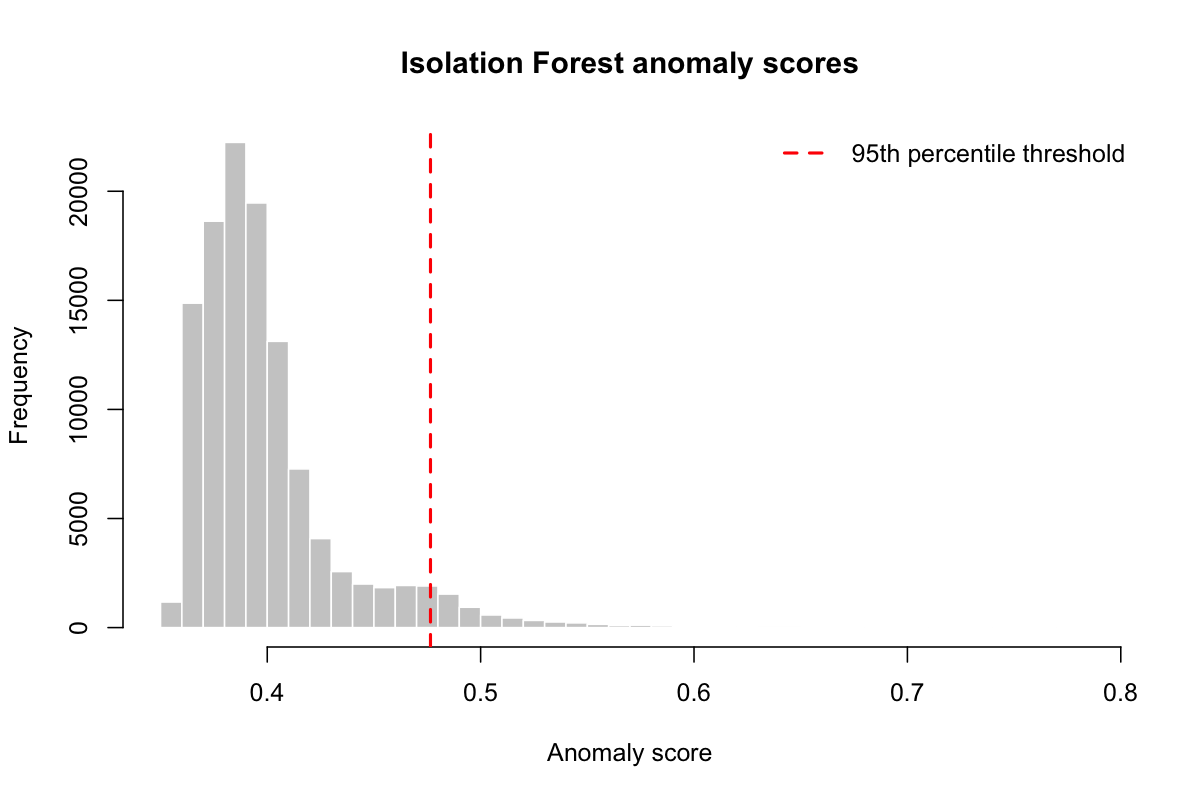
\includegraphics[width=0.85\textwidth]{../plots/01_isolation_forest_scores.png}
\caption{Distribution of Isolation Forest anomaly scores. The dashed line marks the 95th percentile threshold.}
\end{figure}

\section{Bayesian Beta-Binomial Model}

We now model the global anomaly rate $\pi$ as $Y_i \sim \text{Bernoulli}(\pi)$, with prior parameter distribution $\pi \sim \text{Beta}(\alpha_0, \beta_0)$.

This choice is motivated by the conjugacy between the Beta prior and the Bernoulli likelihood. Conjugacy implies that the posterior distribution belongs to the same family as the prior, leading to a closed-form update:

\[
\pi \mid Y \sim \text{Beta}(\alpha_0 + k, \beta_0 + n - k),
\]

where $k = \sum_{i=1}^n Y_i$ is the number of observed anomalies of $n$ observations.

\subsection{Interpretation}

The posterior expectation value with $\alpha=\alpha_0+k$ and $\beta=\beta_0+n-k$ is so:
\[
\mathbb{E}[\pi \mid Y] = \frac{\alpha}{\alpha + \beta}.
\]

The Beta-Binomial analysis is performed on a random subsample of $250$ transactions, in which $13$ anomalies are observed. This corresponds to an empirical anomaly rate of $5.2\%$ in the subsample.

\begin{table}[H]
\centering
\begin{tabular}{lrrrrr}
\toprule
\textbf{Prior} & $\alpha$ & $\beta$ & \textbf{Posterior $\mathbb{E}$} & \textbf{95\% CI low} & \textbf{95\% CI high} \\
\midrule
Beta(1,1) & 14 & 238 & 0.0556 & 0.0308 & 0.0869 \\
Beta(1,19) & 14 & 256 & 0.0519 & 0.0287 & 0.0812 \\
Beta(5,95) & 18 & 332 & 0.0514 & 0.0309 & 0.0769 \\
\bottomrule
\end{tabular}
\caption{Posterior estimates under different Beta priors}
\end{table}

\begin{figure}[H]
\centering
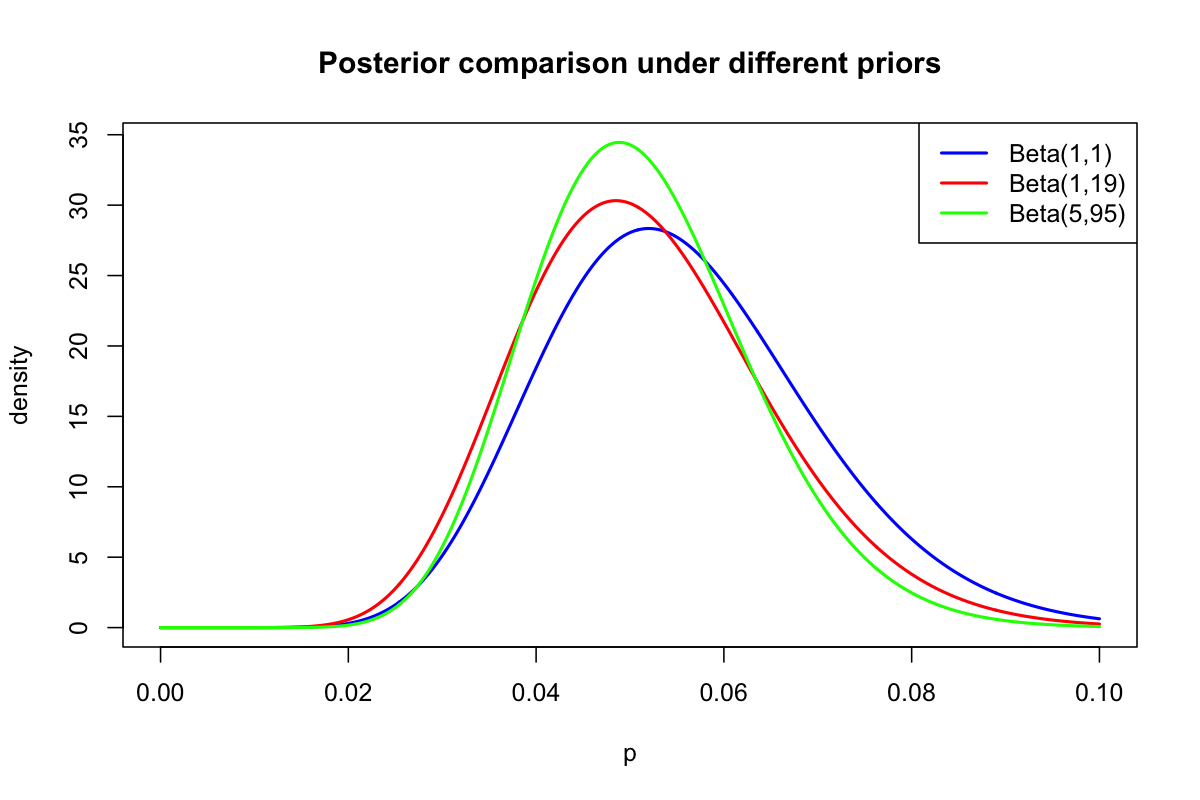
\includegraphics[width=0.85\textwidth]{../plots/02_beta_posterior_comparison.png}
\caption{Posterior distributions of the anomaly probability under three different Beta priors.}
\end{figure}

As the prior becomes more informative, the posterior expectation progressively shifts toward the prior belief of an overall anomaly rate close to \(5\%\). In particular, stronger priors reduce the influence of the sampled observations, leading to posterior estimates that are more concentrated around the prior information and exhibit more concentrated credible intervals.

\section{Sequential Bayesian Learning}

To analyze how the anomaly probability evolves over time, we consider an online update scheme.

At each time step $t$, we update:

\[
\alpha_t = \alpha_0 + k_t, \quad \beta_t = \beta_0 + t - k_t,
\]

where $k_t$ is the cumulative number of anomalies observed up to time $t$.

The posterior expectation evolves as:

\[
\mathbb{E}[\pi_t \mid Y_t] = \frac{\alpha_t}{\alpha_t + \beta_t}.
\]

This allows us to track how the estimated anomaly probability changes as more transactions are observed.

At the end of the sequential updating procedure, the posterior mean anomaly probability is $0.050007$. The final 90\% credible interval is $[0.048960, 0.051063]$, showing that after observing the full sequence the global anomaly rate is estimated very precisely.

\begin{table}[H]
\centering
\begin{tabular}{lr}
\toprule
\textbf{Quantity} & \textbf{Value} \\
\midrule
Final posterior mean & 0.050007 \\
Final 90\% credible interval lower bound & 0.048960 \\
Final 90\% credible interval upper bound & 0.051063 \\
Minimum posterior mean over time & 0.050007 \\
Maximum posterior mean over time & 0.986667 \\
\bottomrule
\end{tabular}
\caption{Sequential Bayesian learning summary}
\end{table}

\begin{figure}[H]
\centering
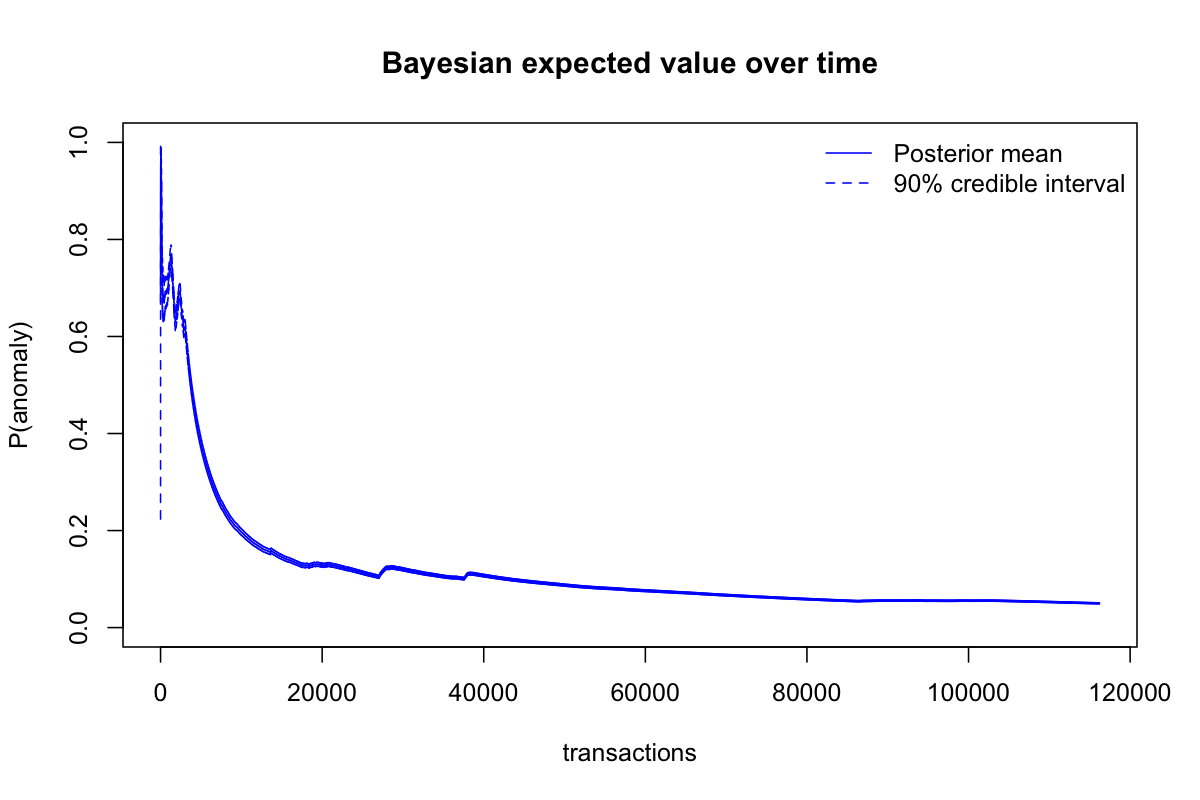
\includegraphics[width=0.85\textwidth]{../plots/03_sequential_bayesian_learning.png}
\caption{Sequential posterior mean of the anomaly probability with 90\% credible interval.}
\end{figure}

\section{Bayesian Logistic Regression via MCMC}

While the Beta-Binomial model provides a global estimate of the anomaly rate, it does not incorporate transaction-level information. To model how transaction characteristics influence the probability of anomalous behaviour, we extend the analysis through Bayesian logistic regression.

Given a binary anomaly indicator $Y_i \in \{0,1\}$ for transaction $i$, we assume $Y_i \sim \text{Bernoulli}(\pi_i)$ where $\pi_i$ represents the probability that transaction $i$ is anomalous. The probability is linked to the observed covariates through a logistic regression model:

\[
\text{logit}(\pi_i) = \log \frac{\pi_i}{1 - \pi_i}
=
\beta_0
+
\beta_1 x_{i1}
+
\beta_2 x_{i2}
+
\beta_3 x_{i3}
+
\beta_4 x_{i4}.
\]

The predictors include standardized transaction amount, standardized balance, standardized log-time, withdrawal indicator, balance-to-amount ratio, and weekday effects.

Differently from the Beta-Binomial setting, the posterior distribution of the regression coefficients cannot be derived analytically due to the non-conjugate logistic likelihood. For this reason, posterior inference is performed through Markov Chain Monte Carlo (MCMC) methods.

\subsection{MCMC intuition}

Instead of producing a single point estimate for the parameters, MCMC generates a sequence of samples:

\[
\beta^{(1)}, \beta^{(2)}, \dots, \beta^{(s)}
\sim
p(\beta \mid Y,X),
\]

which approximate the posterior distribution of the model parameters. Each draw corresponds to one plausible configuration of the regression coefficients given the observed data.

More specifically, each sampled vector contains one coefficient for every feature included in the model $\beta^{(s)}=\left(\beta_0^{(s)},\beta_1^{(s)},...,\beta_n^{(s)}\right)$, where each component represents the effect of a specific transaction feature on the anomaly probability.

The sampling procedure constructs a Markov chain whose stationary distribution coincides with the posterior distribution of the parameters. After an initial warm-up phase, the chain progressively explores the high-probability regions of the posterior space. The objective is to obtain samples that are as weakly correlated as possible, so that successive draws behave approximately as independent realizations from the target posterior distribution.

Predictions are therefore obtained by averaging over many sampled parameter configurations rather than relying on a single estimated model. This allows the Bayesian framework to naturally quantify predictive uncertainty.

In particular, for each transaction the model provides a posterior mean probability of fraud and a credible interval describing uncertainty around the prediction.

This represents one of the main conceptual differences with respect to the frequentist logistic regression approach, which produces only point estimates of the probabilities.

The Bayesian logistic regression was fitted on $92960$ training observations and evaluated on $23241$ test observations. The training anomaly rate is $0.050022$, while the test anomaly rate is $0.049912$.

Three prior specifications were compared for the regression coefficients and intercept: a standard normal prior $\mathcal{N}(0,1)$, a weakly informative normal prior $\mathcal{N}(0,2)$, and a Cauchy$(0,2.5)$ prior. The Cauchy$(0,2.5)$ prior follows the recommendation of Gelman et al. (2008), which is commonly used as a weakly informative default for Bayesian logistic regression.

\begin{table}[H]
\centering
\begin{tabular}{lrrr}
\toprule
\textbf{Prior} & \textbf{Max $\hat{R}$} & \textbf{Min bulk ESS} & \textbf{Min tail ESS} \\
\midrule
Normal(0,1) & 1.003 & 1045.7 & 1251 \\
Cauchy(0,2.5) & 1.003 & 807.8 & 1150 \\
Normal(0,2) & 1.005 & 831.1 & 1318 \\
\bottomrule
\end{tabular}
\caption{MCMC diagnostic summary}
\end{table}

The convergence diagnostics are satisfactory: all fixed-effect $\hat{R}$ values are close to 1, and the effective sample sizes are sufficiently large for the fixed effects.

The regression coefficients can be interpreted on the log-odds scale. For the Cauchy$(0,2.5)$ model, the coefficient of \textit{amount} is positive ($2.05$), meaning that larger standardized transaction amounts increase the posterior probability of being classified as anomalous. In odds terms, a one-standard-deviation increase in amount multiplies the odds by approximately $\exp(2.05) \approx 7.8$, holding the other variables fixed. By contrast, \textit{log\_time} has a negative coefficient ($-1.84$), so later transactions in the sequence are associated with lower anomaly odds, approximately multiplied by $\exp(-1.84) \approx 0.16$. The variable \textit{balance\_amount\_ratio} has a strongly negative coefficient, suggesting that transactions that are large relative to the balance are much more likely to be anomalous.

\section{Comparison of Bayesian Approaches}

The two Bayesian approaches considered in this work address anomaly detection at different levels of complexity.

The Beta-Binomial model provides a simple probabilistic description of the overall anomaly frequency in the dataset. Due to the conjugacy between the Beta prior and the Bernoulli likelihood, posterior inference admits a closed-form solution and can be computed analytically. This makes the model highly interpretable and computationally efficient, although limited to estimating a global anomaly probability.

The Bayesian logistic regression model extends the analysis by incorporating transaction-specific covariates. In this case, posterior inference no longer admits a closed-form expression and requires simulation-based methods such as MCMC. Although computationally more expensive, this approach allows the anomaly probability to vary across transactions according to their observed characteristics.

From a predictive perspective, all Bayesian logistic regressions outperform the frequentist logistic regression in ROC-AUC, log loss, and F1-score when using the fixed threshold $0.5$.

The final Bayesian row in the performance table uses the Cauchy$(0,2.5)$ model, which gives the best AUC and log loss among the Bayesian priors. The only difference is the classification threshold. With the standard threshold $0.5$, the model has precision $0.7849$ and recall $0.6198$. With the ROC-optimal threshold $0.1047$, more observations are classified as anomalies, increasing recall to $0.9491$, but reducing precision to $0.5432$.

Thus, the optimal threshold is better when detecting more anomalies is more important than avoiding false positives. AUC and log loss remain unchanged because they evaluate predicted probabilities, not the final binary classification.

\begin{table}[H]
\centering
\small
\begin{tabular}{lrrrrrr}
\toprule
\textbf{Model} & \textbf{Threshold} & \textbf{AUC} & \textbf{Accuracy} & \textbf{Log loss} & \textbf{Recall} & \textbf{F1} \\
\midrule
Frequentist & 0.50 & 0.9313 & 0.9670 & 0.0966 & 0.4707 & 0.5877 \\
Bayes N(0,1) & 0.50 & 0.9767 & 0.9725 & 0.0680 & 0.6103 & 0.6894 \\
Bayes Cauchy(0,2.5) & 0.50 & 0.9790 & 0.9725 & 0.0674 & 0.6198 & 0.6927 \\
Bayes N(0,2) & 0.50 & 0.9781 & 0.9725 & 0.0675 & 0.6164 & 0.6915 \\
Bayes Cauchy optimal & 0.1047 & 0.9790 & 0.9576 & 0.0674 & 0.9491 & 0.6909 \\
\bottomrule
\end{tabular}
\caption{Predictive performance on the test set}
\end{table}

\begin{table}[H]
\centering
\begin{tabular}{lrrrr}
\toprule
\textbf{Model} & \textbf{TP} & \textbf{TN} & \textbf{FP} & \textbf{FN} \\
\midrule
Frequentist & 546 & 21929 & 152 & 614 \\
Bayes N(0,1) & 708 & 21895 & 186 & 452 \\
Bayes Cauchy(0,2.5) & 719 & 21884 & 197 & 441 \\
Bayes N(0,2) & 715 & 21888 & 193 & 445 \\
Bayes Cauchy optimal & 1101 & 21155 & 926 & 59 \\
\bottomrule
\end{tabular}
\caption{Confusion matrix components on the test set}
\end{table}

\begin{figure}[H]
\centering
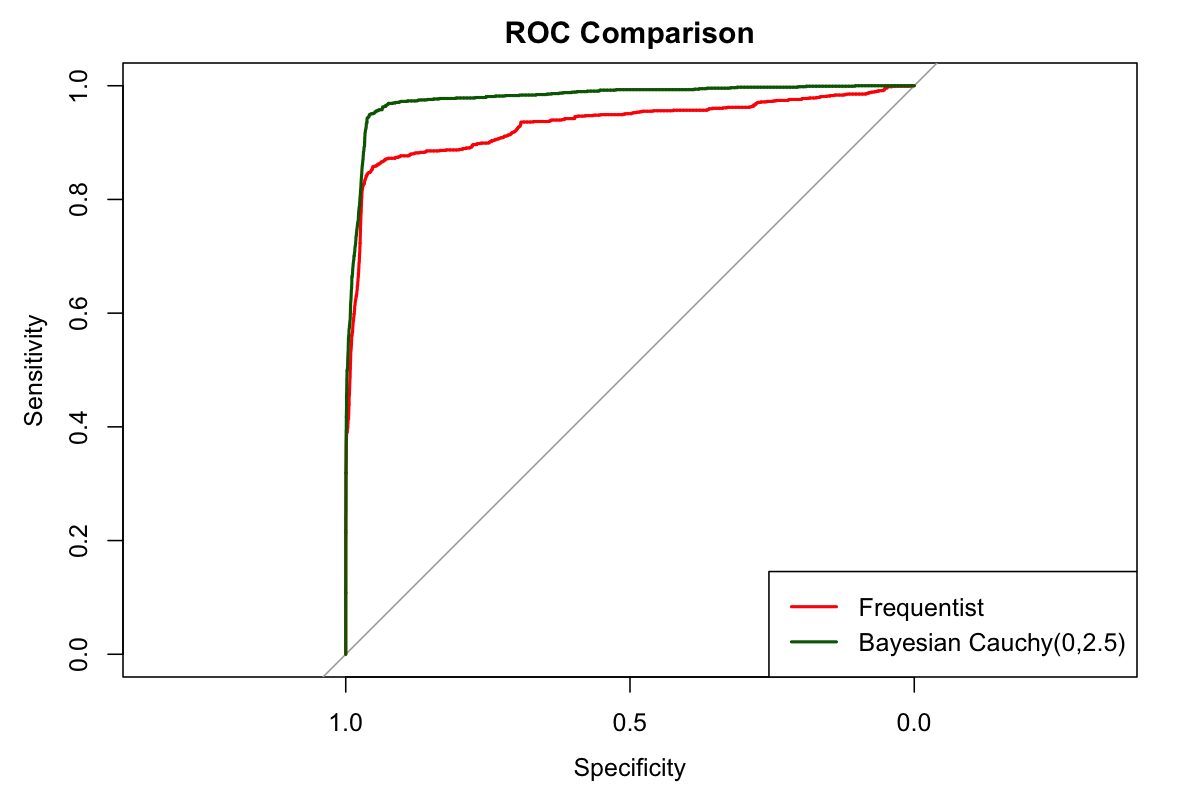
\includegraphics[width=0.85\textwidth]{../plots/04_roc_comparison.png}
\caption{ROC curve comparison between frequentist logistic regression and the Bayesian logistic regression with Cauchy$(0,2.5)$ prior.}
\end{figure}

For the Bayesian model with Cauchy$(0,2.5)$ prior, the posterior predictive probabilities have mean $0.050558$ and median $0.000387$. Their 5\% and 95\% quantiles are $0.000006$ and $0.349947$, respectively. The average width of the 90\% credible interval is $0.005020$, with median width $0.000133$.

\begin{figure}[H]
\centering
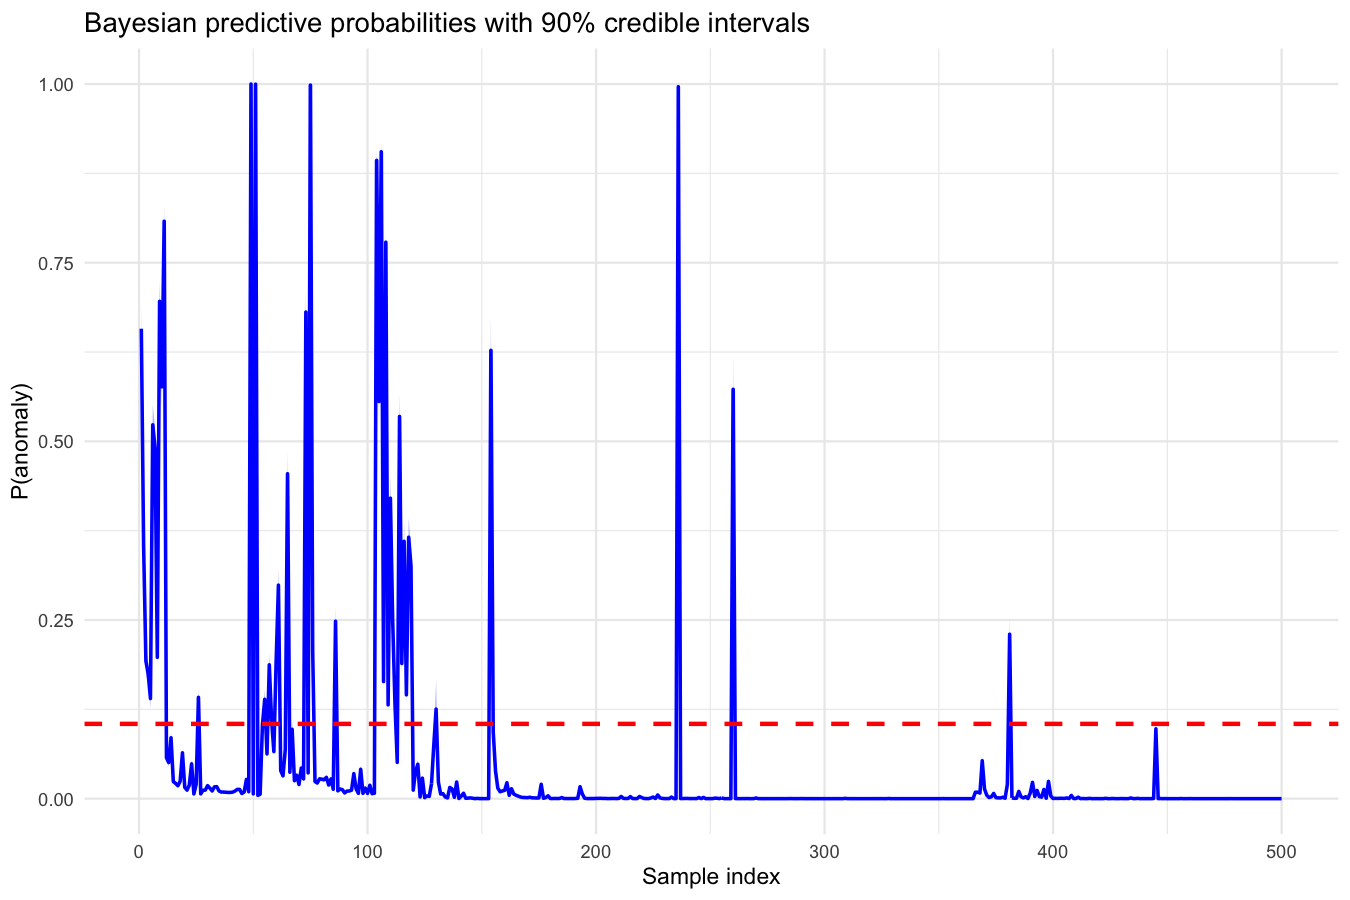
\includegraphics[width=0.85\textwidth]{../plots/05_bayesian_predictive_uncertainty.png}
\caption{Bayesian posterior predictive probabilities with 90\% credible intervals for a sample of test observations.}
\end{figure}

The Bayesian framework therefore provides not only point predictions and classification performance, but also a direct quantification of uncertainty. This additional uncertainty quantification is particularly relevant in fraud detection applications, where identifying uncertain or borderline cases may be as important as maximizing classification accuracy itself.

\section*{References}

Gelman, A., Jakulin, A., Pittau, M. G., and Su, Y.-S. (2008). A weakly informative default prior distribution for logistic and other regression models. \textit{The Annals of Applied Statistics}, 2(4), 1360--1383.

\end{document}
